\documentclass[a4paper,12pt]{article}
\usepackage{graphicx}
\usepackage[UTF8]{ctex}
\usepackage{fontspec}
\usepackage{booktabs}
\usepackage{float}%浮动体
\usepackage{amsmath,amssymb}
\usepackage{fancyhdr}
%\usepackage{xcolor}
\usepackage{colortbl}
\usepackage{geometry}
\geometry{top=2cm,bottom=2cm,left=1cm,right=1cm}
\begin{document}
	\begin{figure}[H]
	\begin{center}
		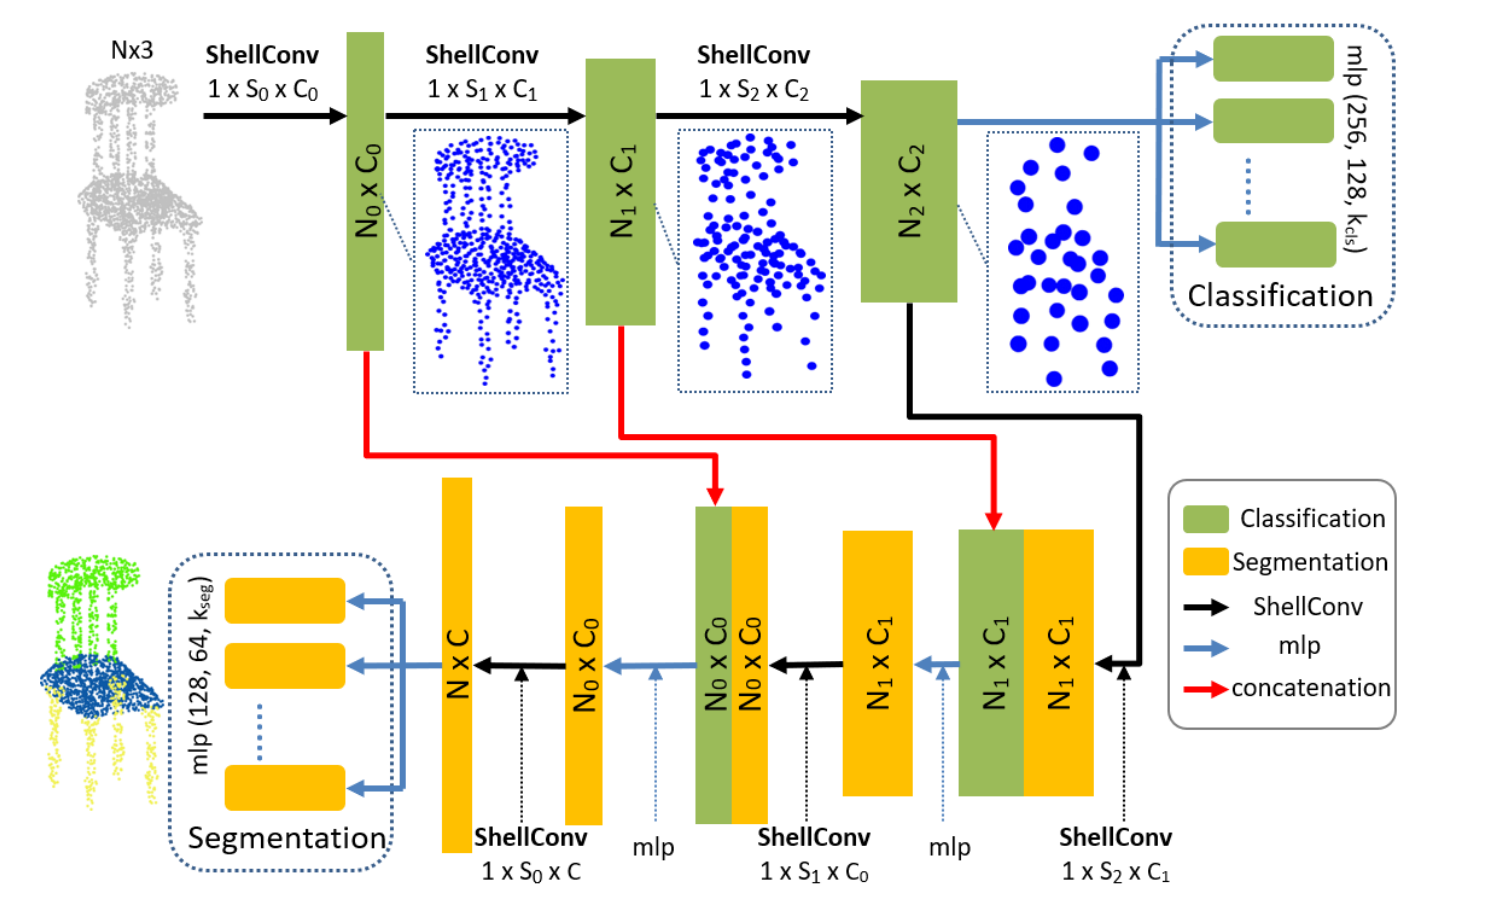
\includegraphics[width=0.9\textwidth]{img/ShellNet.png} 
		\caption{ShellNet}
	\end{center}
\end{figure}

	\begin{figure}[H]
		\begin{center}
			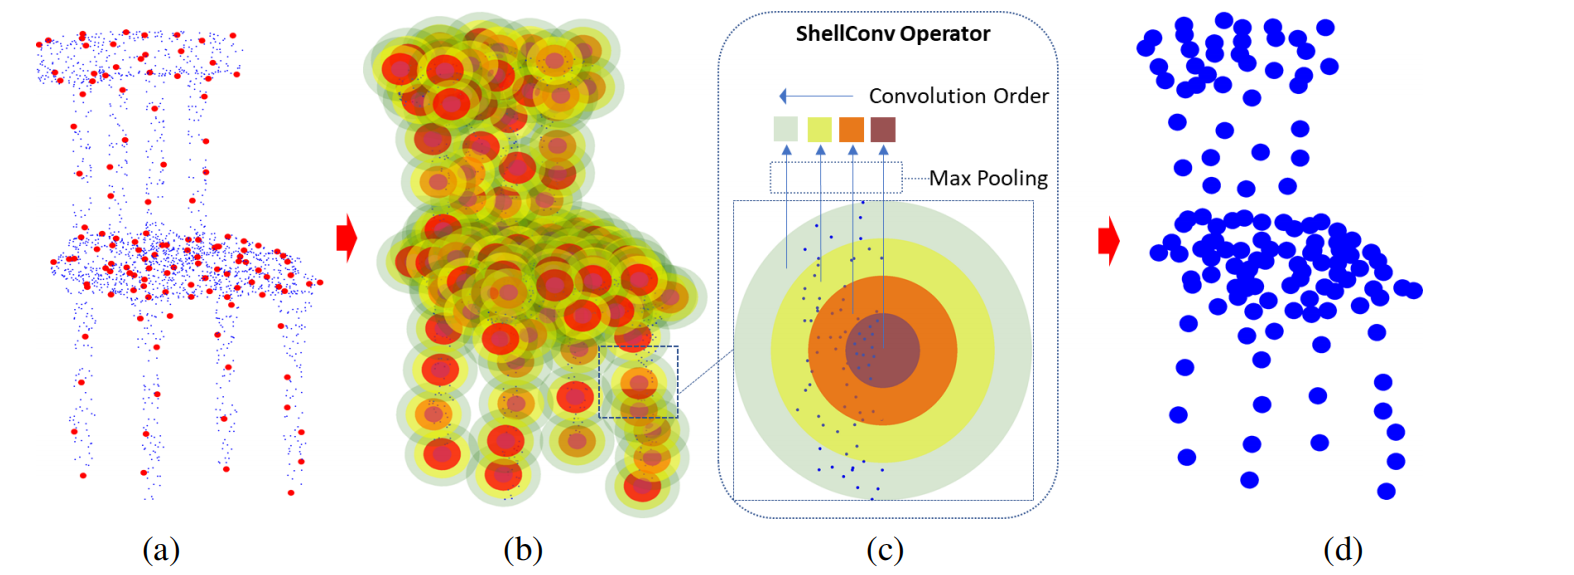
\includegraphics[width=0.9\textwidth]{img/ShellConv.png} 
			\caption{ShellConv}
		\end{center}
	\end{figure}


\textbf{ShellConv}:
\begin{itemize}
	\item 随机采样,图1(a)红点,画圆进行统计。
	\item 每个Shell中的点进行pooling,随后按照Shell顺序进行卷积特征提取
\end{itemize}
	$$
F(p)^{(n)}=\sum_{q \in \Omega_{p}^{(n)}} w(q)^{(n)} F(q)^{(n-1)}
$$

$$
F(p)^{(n)}=\sum_{S \in \Omega_{p}^{(n)}} w_{S}^{(n)} F(S)^{(n-1)}
$$
$$
F(S)=\operatorname{maxpool}\left(\left\{F(q): q \in \Omega_{S}\right\}\right)
$$

\paragraph{分类任务}
特征提取之后,MLP(256,128,$k_{cls}$),进行分类
\paragraph{语义分割} 如图1,使用了"反卷积"(还是以Shell的形式),和跳跃连接。(类似PointNet++)

\end{document}